\section{Technical Overview}
\subsection{Architecture}
Blocktree redefines blockchain as a dynamically growing tree, beginning with a single genesis block where mining initiates, akin to Bitcoin~\cite{nakamoto2008bitcoin}. After an interval on the order of millions of blocks, the initial chain, serving as the root, splits into two fully isolated branches, each continuing as an independent ledger. Subsequent splits occur on these branches periodically, guided by network topology, forming a tree-like structure that expands over time, as illustrated in Figure~\ref{fig:treegrowth}. All branches share a common cryptocurrency, Blocktree Coin (BKT), mined across the network, ensuring economic unity despite isolation. Nodes self-organize into clusters by measuring peer-to-peer latency (e.g., via periodic pings averaged over thousands of blocks), employing a spectral clustering method~\cite{ng2001spectral} to group those with minimal communication delays. The clustering constructs a Laplacian matrix $L = D - A$, where $D$ is the degree matrix and $A$ is the adjacency matrix weighted by inverse latency. At each split interval, the least cohesive cluster is identified using the Fiedler vector—the eigenvector corresponding to the second smallest eigenvalue $\lambda_2$ of $L$. Nodes are partitioned into two branches based on the sign of their Fiedler vector components, reassigning miners to optimize latency proximity, doubling capacity while enhancing spatial efficiency. This hybrid approach—periodic and topology-aware—enables scalability across the solar system or interstellar space, where light-speed delays (e.g., 3–24 minutes Earth-to-Mars) are mitigated by branch autonomy. Branches link to their parent via hash pointers, preserving immutability and decentralization, while parallel validation across the tree supports a theoretically unbounded throughput, potentially exceeding thousands of transactions per second per branch.

\begin{figure}[h]
\centering
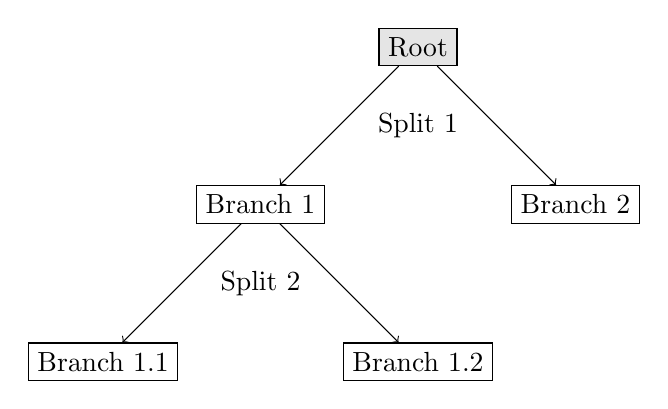
\begin{tikzpicture}
    \node[rectangle, draw, fill=gray!20] (R) at (0,0) {Root};
    \node[rectangle, draw] (B1) at (-2,-2) {Branch 1};
    \node[rectangle, draw] (B2) at (2,-2) {Branch 2};
    \node[rectangle, draw] (B3) at (-4,-4) {Branch 1.1};
    \node[rectangle, draw] (B4) at (0,-4) {Branch 1.2};
    \draw[->] (R) -- (B1);
    \draw[->] (R) -- (B2);
    \draw[->] (B1) -- (B3);
    \draw[->] (B1) -- (B4);
    \node[align=center] at (0,-1) {Split 1};  % Between Root and Branches 1 & 2
    \node[align=center] at (-2,-3) {Split 2};  % Between Branch 1 and Branches 1.1 & 1.2
\end{tikzpicture}
\caption{Blocktree growth, showing periodic split points from the root.}
\label{fig:treegrowth}
\end{figure}

\subsection{Consensus Mechanism}
Blocktree employs a Proof of Work (PoW) consensus protocol to secure its tree structure, prioritizing openness and decentralization~\cite{nakamoto2008bitcoin}. Miners within each branch solve computational puzzles to append blocks, requiring no prior coin ownership—a design that keeps the network permissionless and accessible to any node with computational power. The shared cryptocurrency, BKT, is mined with each block, starting from the genesis, with a constant exponential decrease to regulate supply as branches proliferate. The target block time is subsecond (e.g., 0.2 seconds), enabling high-frequency transactions. Difficulty adjusts dynamically, akin to Bitcoin’s mechanism~\cite{nakamoto2008bitcoin}, recalculating every tens of thousands of blocks to maintain the target block time, regardless of cluster size or miner distribution. Inter-branch coordination is minimal; branches operate independently post-split, relying on PoW for local security, with the genesis block as the currency’s origin. Cross-branch transactions maintain BKT fungibility via miner-validated transfers, ensuring economic activity scales with the tree’s growth while maintaining fairness and resilience in the P2P network.

\subsection{Implementation}
Blocktree’s architecture is designed as a fully decentralized P2P network~\cite{stoica2001chord}, with development focused on realizing its hybrid splitting and spectral clustering mechanisms~\cite{vonluxburg2007tutorial}. The system begins with a single genesis block, initiating a chain that splits into branches periodically, guided by latency-based clusters. Miners form these clusters by measuring peer-to-peer latency, applying a spectral clustering algorithm to construct the Laplacian $L$ and partition the network into cohesive groups, splitting based on the Fiedler vector’s sign structure. Each branch mines BKT independently, creating a self-sustaining economy across isolated segments, with node discovery facilitated by a gossip protocol to handle churn. This open-source initiative invites collaboration to implement live P2P functionality, refine clustering logic for interstellar latencies (e.g., up to 24 minutes), and integrate edge DApps and AI-driven transactions, paving the way for a blockchain that spans the solar system.